

\section{Resumé}
\begin{figure}[h]
	\begin{center}
	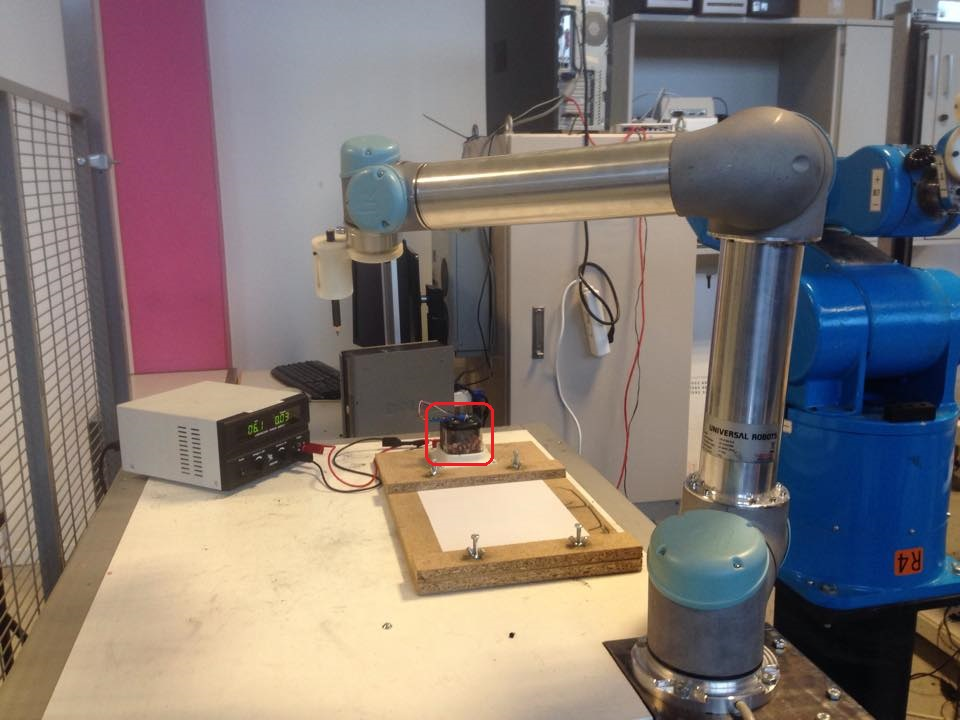
\includegraphics[scale=0.4]{Billeder/UR-farver.jpg}
	\caption{Robotten anvendt til projektet ses holde en blyantspidser, og den modificerede blyantspidser ses i baggrunden af billedet, i den røde boks}\label{fig:opstilling}
	\end{center}
\end{figure}
Projektet omhandler en robot, (se figur ~\ref{fig:opstilling}), der anvendes til at tegne en billede med en blyant samt spidse denne blyant. Det forklares hvordan G-kode, som er et sprog, der fortæller robotten, hvorledes den skal bevæge sig, laves i CAS-værktøjet Mathematica. Den G-kode, som produceres i Mathematica, fortæller robotten, om den skal tegne eller bevæge sig frit i luften samt X-,Y- og Z-koordinater, som beskriver hvor i et tredimentionelt plan, robotten skal være, når den tegner. Foruden dette fortæller det også hvordan billedet skal tegnes, og når robotten skal spidse blyanten. Blyantspidseren, som anvendes i dette projekt er elektrisk og modificeret således, at den automatisk starter når blyanten stikkes i den. I dette elektriske kredsløb er anvendt forskellige komponenter, herunder to forskellige transistorer og en komperator. Det er beskrevet i rapporten hvorledes de anvendte komponenter virker, samt hvilken indflydelse de har i det nye elektriske kredsløb. 
